\newcommand{\quotes}[1]{``#1''}

\section{Objetivos}
\begin{itemize}
    \item Comprender el proceso de Análisis Formal de Conceptos (\textit{FCA}) y su aplicación en la organización jerárquica de datos.
    \item Definir un conjunto de objetos y atributos y construir el látice de conceptos formales correspondiente.
    \item Visualizar y analizar la estructura del látice para interpretar relaciones entre objetos y atributos.
    \item Facilitar la interpretación de los datos a través de la visualización tabular y gráfica.
\end{itemize}

\section{Marco Teórico}

El Análisis Formal de Conceptos (\textit{FCA}, por sus siglas en inglés) es un enfoque matemático para analizar y estructurar datos a partir de conceptos formales. Un \textbf{concepto formal} se define como un par de conjuntos: la \textbf{extensión}, que representa los objetos que cumplen ciertos atributos, y la \textbf{intensión}, que es el conjunto de atributos que comparten dichos objetos. El conjunto de todos los conceptos formales de un contexto, junto con la relación de subconjunto entre sus extensiones, forma una estructura jerárquica llamada \textbf{látice de conceptos}.\\


El \textit{FCA} permite identificar relaciones y patrones en datos binarios y representa estas relaciones en un látice que muestra la inclusión de subconjuntos entre conceptos. Los nodos en el látice representan conceptos y las conexiones representan relaciones de subconjunto, donde los conceptos más generales están en niveles superiores y los específicos en niveles inferiores. Este tipo de análisis es útil para explorar y organizar datos en una variedad de áreas, como la ciencia de la información, el aprendizaje automático y la biología.

\section{Conjunto de Objetos con sus Atributos}

Definimos un conjunto de \textbf{objetos} y \textbf{atributos} para el análisis formal. Estos objetos y atributos representan un contexto formal para el análisis.

\begin{itemize}
  \item \textbf{Objetos}:
  \begin{itemize}
      \item O1: \quotes{Libro de Ciencia}
      \item O2: \quotes{Cuaderno}
      \item O3: \quotes{Bolígrafo}
      \item O4: \quotes{Regla}
      \item O5: \quotes{Lápiz}
      \item O6: \quotes{Libro de Matemáticas}
      \item O7: \quotes{Calculadora}
      \item O8: \quotes{Compás}
  \end{itemize}
\end{itemize}

\begin{itemize}
  \item \textbf{Atributos}:
  \begin{itemize}
      \item A1: \quotes{Escribible}
      \item A2: \quotes{Leíble}
      \item A3: \quotes{De medición}
      \item A4: \quotes{Digital}
      \item A5: \quotes{De dibujo}
  \end{itemize}
\end{itemize}

\section{Descripción del Contexto Formal}

La descripción detallada de cada objeto con sus atributos es la siguiente:

\begin{itemize}
    \item \textbf{O1} (\quotes{Libro de Ciencia}) - Atributos: Leíble
    \item \textbf{O2} (\quotes{Cuaderno}) - Atributos: Escribible, Leíble
    \item \textbf{O3} (\quotes{Bolígrafo}) - Atributos: Escribible
    \item \textbf{O4} (\quotes{Regla}) - Atributos: De medición
    \item \textbf{O5} (\quotes{Lápiz}) - Atributos: Escribible
    \item \textbf{O6} (\quotes{Libro de Matemáticas}) - Atributos: Leíble
    \item \textbf{O7} (\quotes{Calculadora}) - Atributos: Digital
    \item \textbf{O8} (\quotes{Compás}) - Atributos: De medición, De dibujo
\end{itemize}

Esta información se presenta en una tabla de contexto formal, donde cada celda indica la presencia (1) o ausencia (0) de un atributo en cada objeto (Figura \ref{fig:tabular_view}).

\begin{figure}[H]
  \centering
  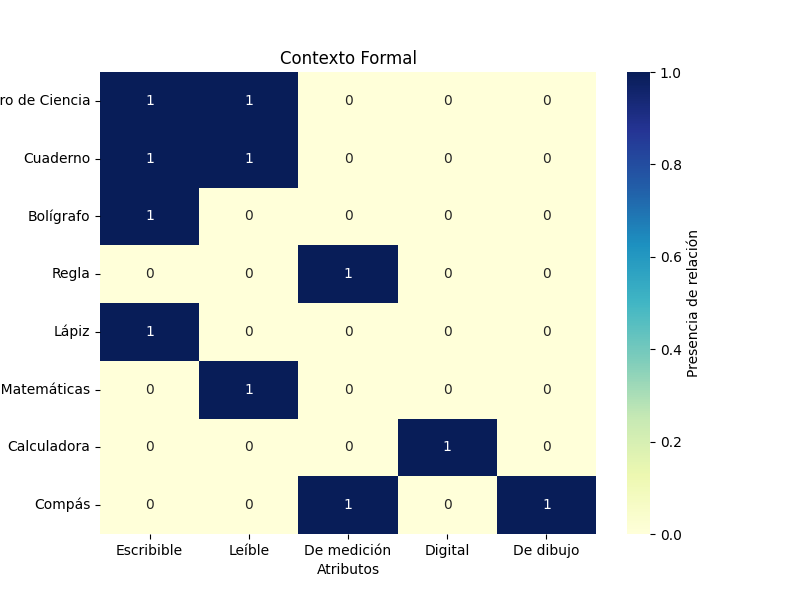
\includegraphics[width=\textwidth]{Figures/1. Content/tabular_view.png}
  \caption{Vista Tabular del Contexto Formal}
  \label{fig:tabular_view}
\end{figure}

\section{Conjunto de Conceptos Formales}

Cada concepto formal \( C \) consiste en un \textbf{conjunto de objetos} (extensión) y un \textbf{conjunto de atributos compartidos} (intensión). A continuación, se presentan algunos conceptos formales extraídos del contexto:

\begin{itemize}
    \item \textbf{C1}: Extensión: \{O1, O2, O6\}, Intensión: \{Leíble\}
    \item \textbf{C2}: Extensión: \{O2\}, Intensión: \{Escribible, Leíble\}
    \item \textbf{C3}: Extensión: \{O3, O5\}, Intensión: \{Escribible\}
    \item \textbf{C4}: Extensión: \{O4\}, Intensión: \{De medición\}
    \item \textbf{C5}: Extensión: \{O7\}, Intensión: \{Digital\}
    \item \textbf{C6}: Extensión: \{O8\}, Intensión: \{De medición, De dibujo\}
    \item \textbf{C7}: Extensión: \{O4, O8\}, Intensión: \{De medición\}
\end{itemize}

\section{Relación de Orden Parcial}

La relación de orden parcial entre los conceptos formales se establece mediante la inclusión de subconjuntos entre extensiones e intensiones. En esta jerarquía, los conceptos específicos (con más atributos) se encuentran en niveles inferiores, mientras que los conceptos más generales (con menos atributos) están en niveles superiores.

\begin{itemize}
    \item \textbf{C1} $\leq$ \textbf{C2}: {O2} es un subconjunto de {O1, O2, O6} y {Escribible, Leíble} $\subseteq$ {Leíble}.
    \item \textbf{C4 $\leq$ C7}: {O4} $\subseteq$ {O4, O8} y {De medición} $\subseteq$ {De medición}.
  \end{itemize}
  

\section{Descripción del Conjunto \( C \) por Extensión}

  El conjunto \( C \) representa todos los conceptos formales generados a partir del contexto formal definido por los objetos y atributos. Cada concepto formal está compuesto por un conjunto de objetos (extensión) y un conjunto de atributos compartidos (intensión).
  
  \subsection{Objetos y Atributos}
  \begin{itemize}
      \item \textbf{O1}: Escribible, Leíble
      \item \textbf{O2}: Escribible, Leíble
      \item \textbf{O3}: Escribible
      \item \textbf{O4}: De medición
      \item \textbf{O5}: Escribible
      \item \textbf{O6}: Leíble
      \item \textbf{O7}: Digital
      \item \textbf{O8}: De medición, De dibujo
  \end{itemize}
  
  \subsection{Conjunto \( C \)}
  El conjunto \( C \) se construye considerando las combinaciones posibles de extensiones e intensiones, sin repeticiones. Incluye las uniones de objetos con las intersecciones de atributos, y viceversa:
  
  \[
  C = \{
  \begin{aligned}
  & (O1; \text{Escribible, Leíble}), (O2; \text{Escribible, Leíble}), (O3; \text{Escribible}), \\
  & (O4; \text{De medición}), (O5; \text{Escribible}), (O6; \text{Leíble}), (O7; \text{Digital}), (O8; \text{De medición, De dibujo}), \\
  & (O1, O2; \text{Escribible, Leíble}), (O1, O6; \text{Leíble}), (O3, O5; \text{Escribible}), (O4, O8; \text{De medición}), \\
  & (O1, O2, O6; \text{Leíble}), (O1, O2, O3, O5; \text{Escribible}), \\
  & (O1, O2, O3, O4, O5, O6, O7, O8; \varnothing), (\varnothing; \text{Escribible, Leíble, De medición, Digital, De dibujo})
  \end{aligned}
  \}
  \]
  
  \subsection{Detalle de los Elementos}
  \begin{itemize}
      \item \( (O1; \text{Escribible, Leíble}) \): El objeto \( O1 \) tiene los atributos \quotes{Escribible} y \quotes{Leíble}.
      \item \( (O8; \text{De medición, De dibujo}) \): El objeto \( O8 \) tiene los atributos\quotes{De medición} y \quotes{De dibujo}.
      \item \( (O3, O5; \text{Escribible}) \): Los objetos \( O3 \) y \( O5 \) comparten el atributo \quotes{Escribible}.
      \item \( (O4, O8; \text{De medición}) \): Los objetos \( O4 \) y \( O8 \) comparten el atributo \quotes{De medición}.
      \item \( (O1, O2, O6; \text{Leíble}) \): Los objetos \( O1, O2 \) y \( O6 \) comparten el atributo \quotes{Leíble}.
      \item \( (O1, O2, O3, O5; \text{Escribible}) \): Los objetos \( O1, O2, O3 \) y \( O5 \) comparten el atributo \quotes{Escribible}.
      \item \( (\varnothing; \text{Escribible, Leíble, De medición, Digital, De dibujo}) \): Conjunto vacío de objetos con todos los atributos.
      \item \( (O1, O2, O3, O4, O5, O6, O7, O8; \varnothing) \): Conjunto completo de objetos sin atributos en común.
  \end{itemize}
  
  Este conjunto \( C \) proporciona una representación jerárquica de todas las posibles combinaciones de relaciones entre los objetos y los atributos, sirviendo como base para la construcción del lattice de conceptos.

\section{Representación Gráfica del Látice del conjunto  \( C \)}
Representación gráfica de los nodos del látice:

\begin{figure}[H]
  \centering
  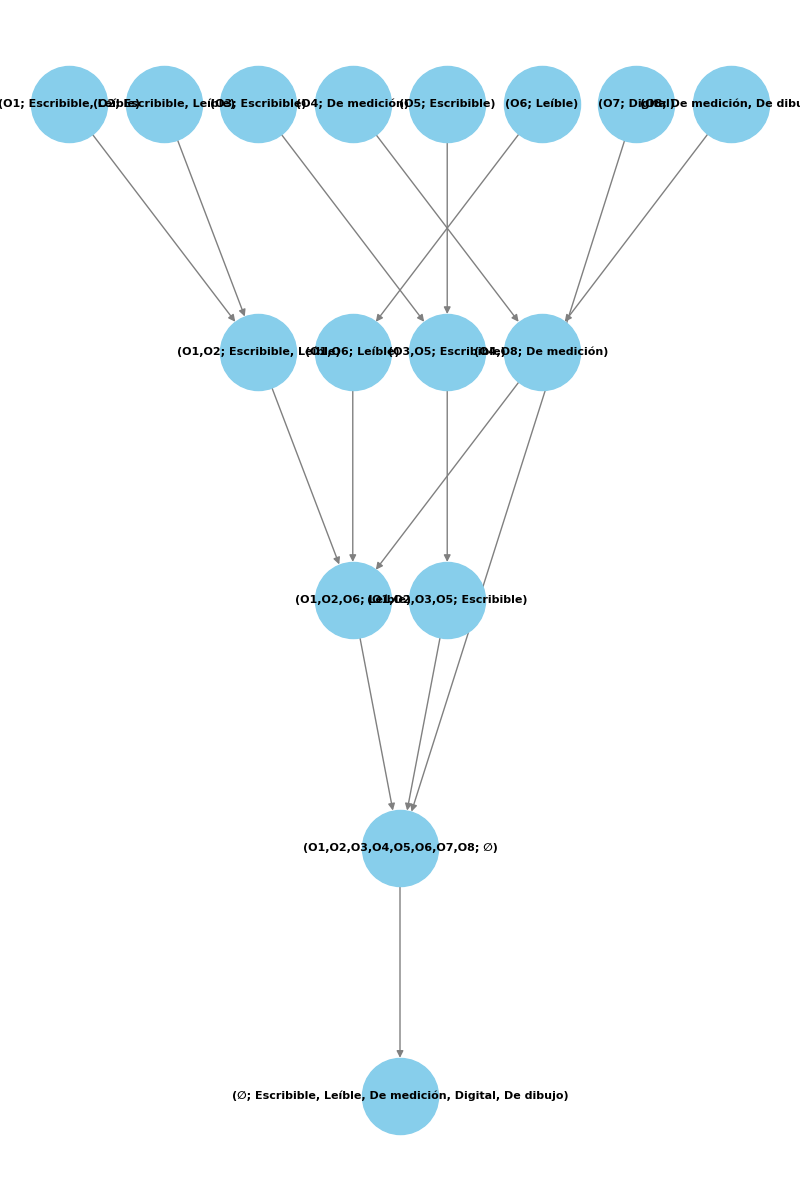
\includegraphics[width=0.8\textwidth]{Figures/1. Content/c_set_lattice_vertical.png}
  \caption{Látice de Conceptos del conjunto  \( C \)}
  \label{fig:c_set_lattice_vertical}
\end{figure}
  
\section{Representación Gráfica del Látice de Conceptos}

La estructura jerárquica de los conceptos se visualiza en un \textbf{Látice de conceptos} (Figura \ref{fig:lattice_view}), donde cada nodo representa un concepto formal y las conexiones muestran las relaciones de inclusión.

\begin{figure}[H]
  \centering
  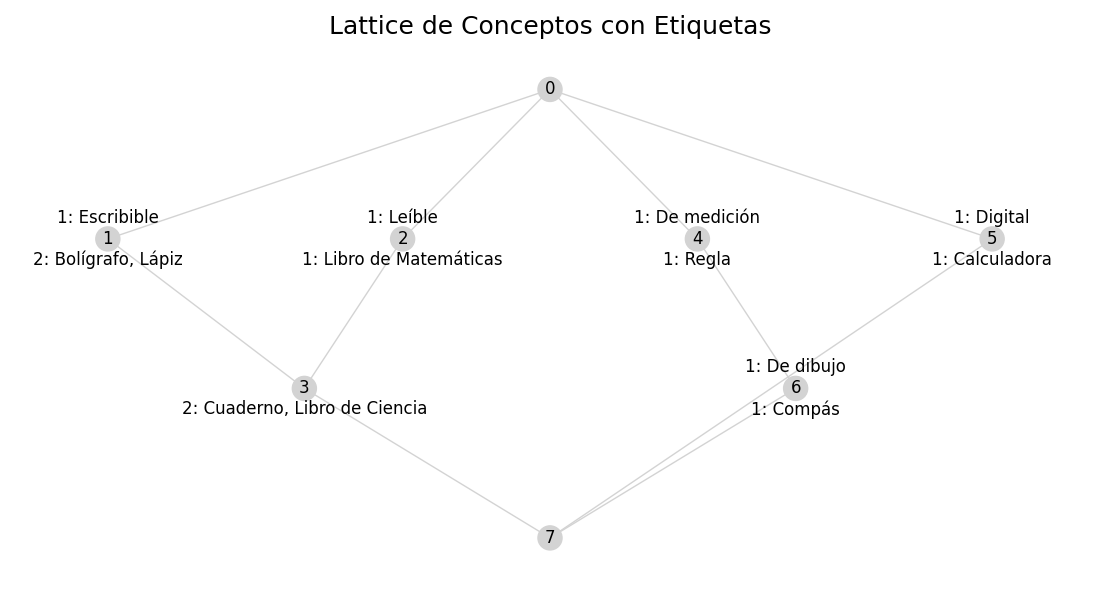
\includegraphics[width=\textwidth]{Figures/1. Content/lattice_view.png}
  \caption{Látice de Conceptos con Etiquetas}
  \label{fig:lattice_view}
\end{figure}

En el Látice:
\begin{itemize}
    \item \textbf{C0} representa el concepto vacío en la parte superior.
    \item Los nodos están etiquetados con el conjunto de atributos o el conjunto de objetos que representan, destacando las relaciones de subconjunto.
\end{itemize}

\section{Conclusiones}

El Análisis Formal de Conceptos permite organizar y visualizar de manera jerárquica la relación entre conjuntos de objetos y atributos en un contexto formal. A través de la construcción de un látice de conceptos, se facilita la interpretación de las relaciones entre datos, destacando las propiedades compartidas y las diferencias entre los objetos. La representación tabular y gráfica ofrece una visión completa del contexto, permitiendo observar tanto la especificidad como la generalidad de los conceptos. Este análisis tiene aplicaciones en diversas disciplinas, proporcionando una estructura útil para el análisis de datos en áreas como la biología, el aprendizaje automático y la organización de información.
